\documentclass[man]{apa6}
\usepackage{lmodern}
\usepackage{amssymb,amsmath}
\usepackage{ifxetex,ifluatex}
\usepackage{fixltx2e} % provides \textsubscript
\ifnum 0\ifxetex 1\fi\ifluatex 1\fi=0 % if pdftex
  \usepackage[T1]{fontenc}
  \usepackage[utf8]{inputenc}
\else % if luatex or xelatex
  \ifxetex
    \usepackage{mathspec}
  \else
    \usepackage{fontspec}
  \fi
  \defaultfontfeatures{Ligatures=TeX,Scale=MatchLowercase}
\fi
% use upquote if available, for straight quotes in verbatim environments
\IfFileExists{upquote.sty}{\usepackage{upquote}}{}
% use microtype if available
\IfFileExists{microtype.sty}{%
\usepackage{microtype}
\UseMicrotypeSet[protrusion]{basicmath} % disable protrusion for tt fonts
}{}
\usepackage{hyperref}
\hypersetup{unicode=true,
            pdftitle={New Lab 8 Title},
            pdfauthor={Angela Lee, Ruby Cuellar, \& Ellen Huang},
            pdfkeywords={psychology, rmarkdown, data science},
            pdfborder={0 0 0},
            breaklinks=true}
\urlstyle{same}  % don't use monospace font for urls
\usepackage{graphicx,grffile}
\makeatletter
\def\maxwidth{\ifdim\Gin@nat@width>\linewidth\linewidth\else\Gin@nat@width\fi}
\def\maxheight{\ifdim\Gin@nat@height>\textheight\textheight\else\Gin@nat@height\fi}
\makeatother
% Scale images if necessary, so that they will not overflow the page
% margins by default, and it is still possible to overwrite the defaults
% using explicit options in \includegraphics[width, height, ...]{}
\setkeys{Gin}{width=\maxwidth,height=\maxheight,keepaspectratio}
\IfFileExists{parskip.sty}{%
\usepackage{parskip}
}{% else
\setlength{\parindent}{0pt}
\setlength{\parskip}{6pt plus 2pt minus 1pt}
}
\setlength{\emergencystretch}{3em}  % prevent overfull lines
\providecommand{\tightlist}{%
  \setlength{\itemsep}{0pt}\setlength{\parskip}{0pt}}
\setcounter{secnumdepth}{0}
% Redefines (sub)paragraphs to behave more like sections
\ifx\paragraph\undefined\else
\let\oldparagraph\paragraph
\renewcommand{\paragraph}[1]{\oldparagraph{#1}\mbox{}}
\fi
\ifx\subparagraph\undefined\else
\let\oldsubparagraph\subparagraph
\renewcommand{\subparagraph}[1]{\oldsubparagraph{#1}\mbox{}}
\fi

%%% Use protect on footnotes to avoid problems with footnotes in titles
\let\rmarkdownfootnote\footnote%
\def\footnote{\protect\rmarkdownfootnote}


  \title{New Lab 8 Title}
    \author{Angela Lee\textsuperscript{1}, Ruby Cuellar\textsuperscript{1}, \& Ellen
Huang\textsuperscript{1}}
    \date{}
  
\shorttitle{lab8}
\affiliation{
\vspace{0.5cm}
\textsuperscript{1} University of Oregon}
\keywords{psychology, rmarkdown, data science}
\usepackage{csquotes}
\usepackage{upgreek}
\captionsetup{font=singlespacing,justification=justified}

\usepackage{longtable}
\usepackage{lscape}
\usepackage{multirow}
\usepackage{tabularx}
\usepackage[flushleft]{threeparttable}
\usepackage{threeparttablex}

\newenvironment{lltable}{\begin{landscape}\begin{center}\begin{ThreePartTable}}{\end{ThreePartTable}\end{center}\end{landscape}}

\makeatletter
\newcommand\LastLTentrywidth{1em}
\newlength\longtablewidth
\setlength{\longtablewidth}{1in}
\newcommand{\getlongtablewidth}{\begingroup \ifcsname LT@\roman{LT@tables}\endcsname \global\longtablewidth=0pt \renewcommand{\LT@entry}[2]{\global\advance\longtablewidth by ##2\relax\gdef\LastLTentrywidth{##2}}\@nameuse{LT@\roman{LT@tables}} \fi \endgroup}


\DeclareDelayedFloatFlavor{ThreePartTable}{table}
\DeclareDelayedFloatFlavor{lltable}{table}
\DeclareDelayedFloatFlavor*{longtable}{table}
\makeatletter
\renewcommand{\efloat@iwrite}[1]{\immediate\expandafter\protected@write\csname efloat@post#1\endcsname{}}
\makeatother

\authornote{

Correspondence concerning this article should be addressed to Angela
Lee, 1451 Onyx Street, Eugene, OR 97403. E-mail:
\href{mailto:alee12@uoregon.edu}{\nolinkurl{alee12@uoregon.edu}}}

\abstract{
Soon our \emph{\textbf{awesome}} abstract will go here.


}

\begin{document}
\maketitle

\section{Commit 3}\label{commit-3}

Cognitive behavioral therapy (CBT) is one of the most effective
psychotherapies for psychological disorders (Zettle \& Hayes, 2015).
Trauer et al. (2015) conducted a meta-analysis on the efficacy of CBT
for insomnia.

\section{Results}\label{results}

\begin{table}[H]
\centering
\begin{tabular}{l|l|r|r|r|r}
\hline
sex & frl & math\_mean & math\_sd & rdg\_mean & rdg\_sd\\
\hline
boy & no & 492.8523 & 46.33845 & 441.4553 & 32.31828\\
\hline
boy & yes & 469.8716 & 46.09285 & 425.3794 & 26.62931\\
\hline
girl & no & 501.2057 & 45.96210 & 448.5353 & 34.52403\\
\hline
girl & yes & 477.5084 & 46.30459 & 430.8029 & 27.42125\\
\hline
\end{tabular}
\end{table}

The mean math score and standard deviation for boys under the no frl
condition was 492.85 and 46.34, respectively. The mean math score and
standard deviation for boys under the yes frl condition was 469.87 and
46.09, respectively. The mean math score and standard deviation for
girls under the no frl condition was 501.21 and 45.96, respectively.
Finally, the mean math score and standard deviation for girls under the
yes frl condition was 477.51 and 46.30, respectively.

\newpage

\section{References}\label{references}

\begingroup
\setlength{\parindent}{-0.5in} \setlength{\leftskip}{0.5in}

\hypertarget{refs}{}
\hypertarget{ref-trauer2015CBT}{}
Trauer, J. M., Qian, M. Y., Doyle, J. S., Rajaratnam, S. M., \&
Cunnington, D. (2015). Cognitive behavioral therapy for chronic
insomnia: A systematic review and meta-analysis. \emph{Annals of
Internal Medicine}, \emph{163}(3), 191--204.

\hypertarget{ref-zettle2015}{}
Zettle, R. D., \& Hayes, S. C. (2015). Rule-governed behavior: A
potential theoretical framework for cognitive-behavioral therapy. In
\emph{The act in context} (pp. 33--63). Routledge.

\endgroup

\newpage

\section{Commit 5}\label{commit-5}

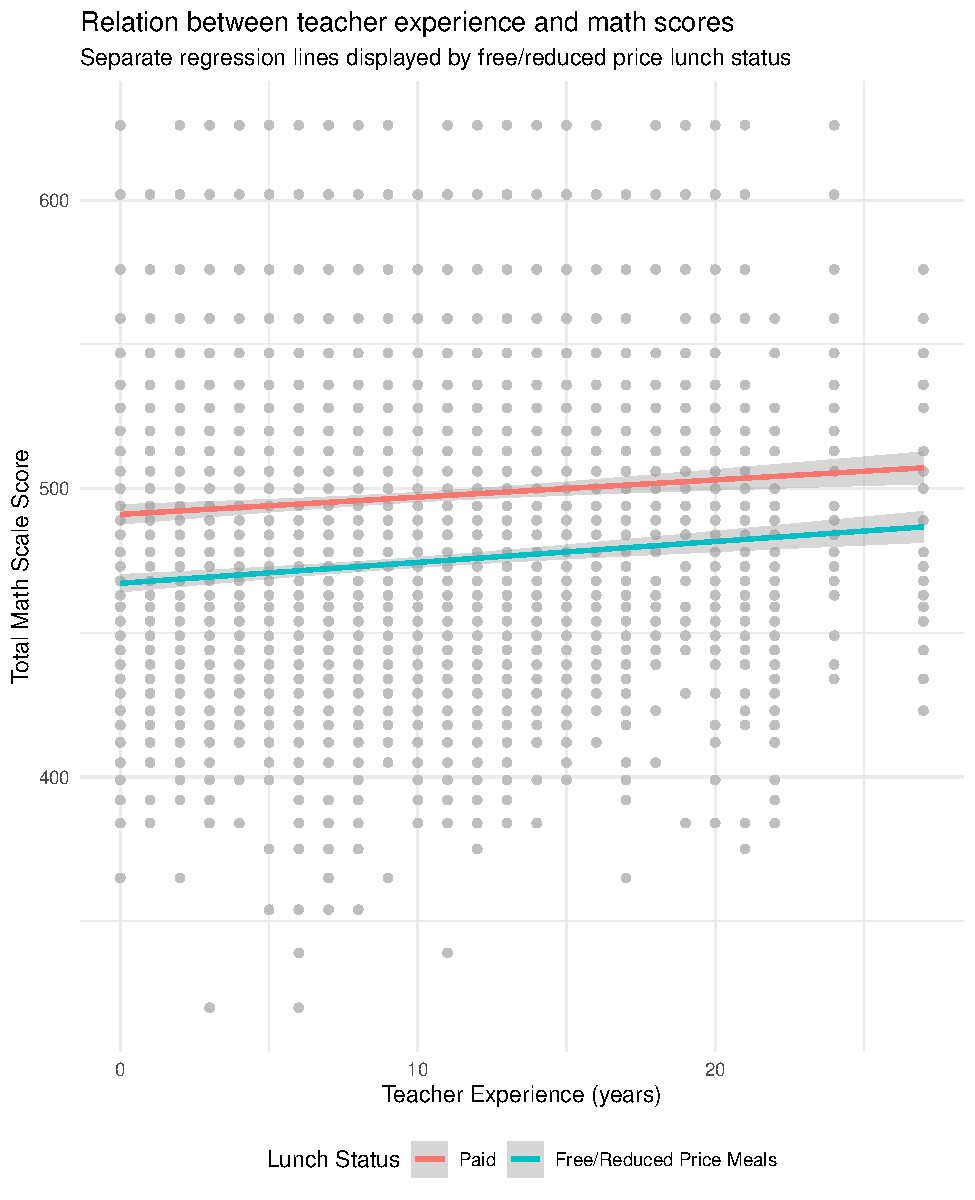
\includegraphics{lab_8_files/figure-latex/unnamed-chunk-2-1.pdf}
\newpage
The graph demonstrates that students who pay for their lunch have higher
total math scale scores than students who receive free or reduced lunch.
We can also see a slight increase in students' math scores if they havea
teacher with more years of teaching experience.


\end{document}
